\section{視線追跡モデルを開発した理由}
近年、AI技術が急速に進化し、画像から様々な情報を取得することが可能になりました。たとえば、物体検出の分野では、Yoloなどの様々なモデルによって、カメラ画像から人や物体の位置をすばやく検出できるようになっています。こうした技術を利用し、視線の位置を特定することができれば、視線を利用した新しい操作インターフェースを提供できるのではないかと考えました。

本プロジェクトの目的は、カメラで取得した視線情報をもとに画面上のカーソルを操作するシステムを開発し、ユーザーが手を使わずに目線のみで操作できる新しいインターフェース体験を提供することです。

\section{全体像}
まず初めに、今回開発した「視線で操作するマウスカーソル」のアプリの全体像について説明していきます。

このアプリでは以下の流れによってユーザーの見ている場所にマウスカーソルを動かします。\\
$\blacksquare$\textbf{マウスカーソルを見ている場所に動かす流れ}
\begin{enumerate}
    \item 4隅を見た時のユーザーの顔画像Tを、PCに内蔵されてあるカメラから取得
    \item TからモデルがPC上で見ている座標を予測し、取得した座標を基に射影変換行列Wを作成
    \item 一定間隔でカメラから顔画像を取得し、顔画像からモデルが予測した座標とWを元に、PC上で見ている座標を予測
    \item 3で予測した座標にマウスカーソルを動かす
    \item 3~4を繰り返し、リアルタイムで見ている場所にマウスカーソルを動かし続ける
\end{enumerate}
射影変換行列Wは「Tから予測した座標を元にモデルが予測したPCの4隅の座標から作られたPCの概形」を「実際のPCの概形」に変換するための行列です。
ここWを用いた理由は、PC上で見ている座標をモデルが予測しても、モデルが予測した座標の単位と実際のPCにおける座標の単位は異なりうるので合わせる必要があるためです。
また、本モデルによる顔画像からのPC上で見ている座標の予測の流れは以下の通りです。\\
\clearpage
$\blacksquare$\textbf{座標予測の流れ}
\begin{enumerate}
    \item 目の位置を推定
    \item 視線の角度を推定
    \item 1.と2.で取得した「視線の角度・目の位置」をもとに、PC上で見ている箇所を計算
\end{enumerate}
以降では、$\blacksquare$\textbf{モデルの推論の流れ}にて言及した「目の位置の推定」と「視線の角度の推定」を行う手順、そして最終的なアプリによる視線の予測結果について説明していきたいと思います。
\section{目の位置の推定}
このモデルは、顔画像から目の位置をPnP問題として考え、推定するモデルです。PnP問題とは「カメラの情報(実際のカメラの位置・やカメラの焦点距離・歪み係数)」と「画面上の物体ととある座標系$D_{world}$(≠カメラを原点とする座標系$D_{camera}$)における物体の位置の関係性」を元に、実際のカメラの位置と回転方向を求める問題です。
\begin{figure}[!ht]
    \centering
    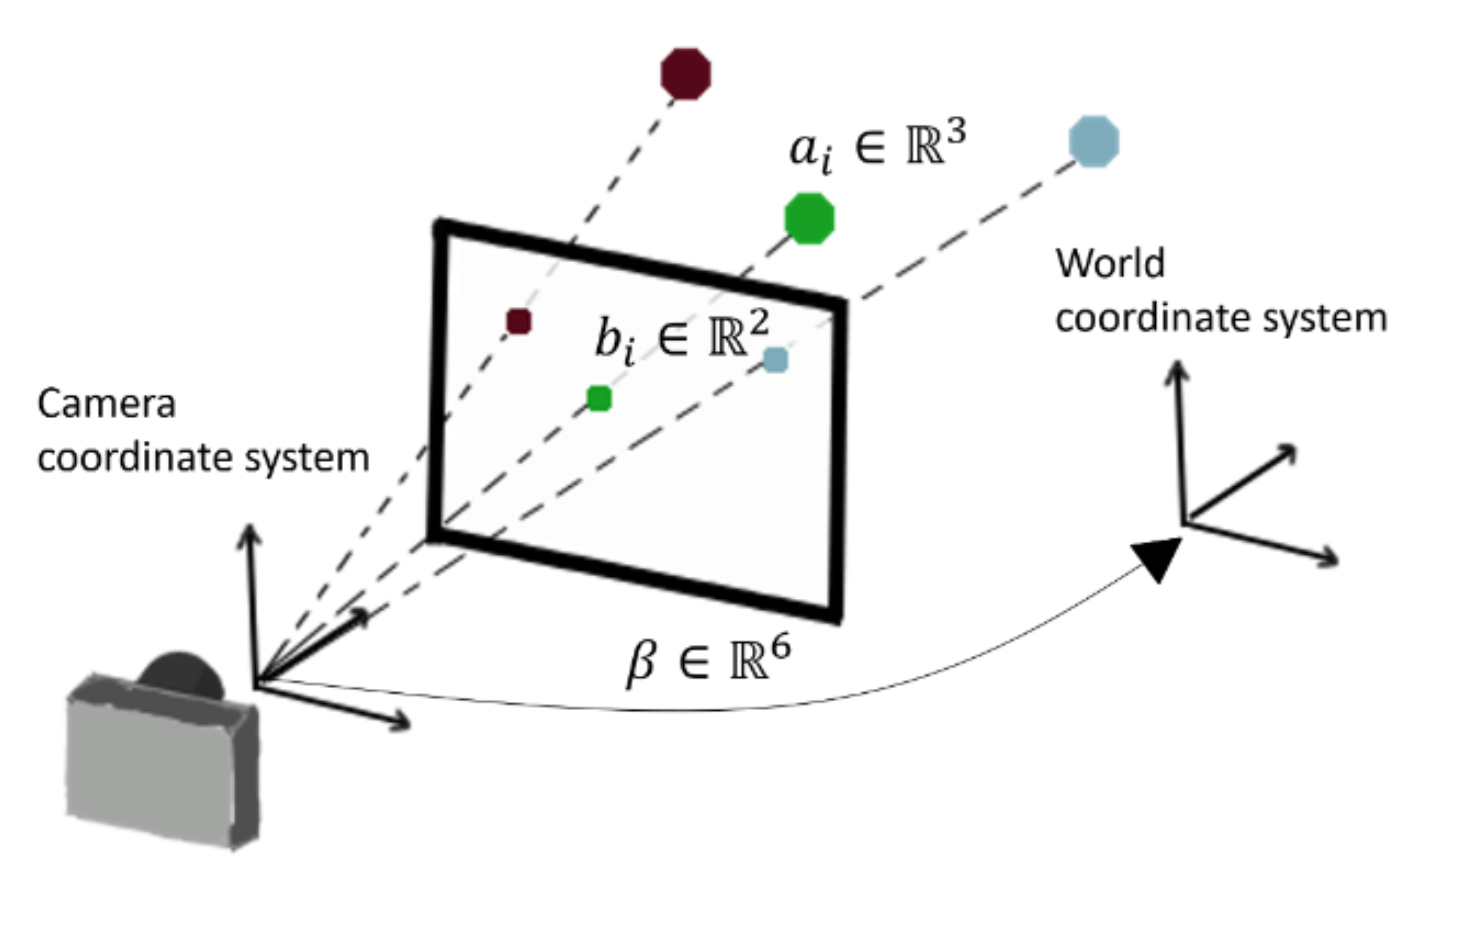
\includegraphics[width=0.7\textwidth]{eye-track-cursor/fig/camera_world_coordinate.png}
    \caption{Camera coordinate system($D_{camera}$)とWorld coordinate system($D_{world}$)の関係性}
    \label{fig:camera_world_coordinate}
\end{figure}
\begin{figure}[!ht]
    \centering
    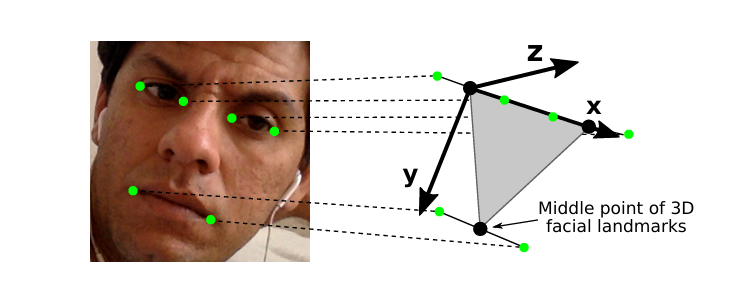
\includegraphics[width=0.7\textwidth]{eye-track-cursor/fig/world_coordinate.png}
    \caption{World coordinate system($D_{world}$)上における顔の特徴点}
    \label{fig:world_coordinate}
\end{figure}
また、顔画像から目の位置を求める流れは以下の通りで、\cite{zhang2017mpiigaze}を元に作成しました。\\
$\blacksquare$\textbf{目の位置を推定する流れ}
\begin{enumerate}
    \item dlibを使用し、画像上における顔の特徴的な部分(目や鼻など)を検出
    \item 「カメラの情報(実際のカメラの位置やカメラの焦点距離・歪み係数)」と「1.で検出した特徴点と$D_{world}$上での一般的な顔における関係性」をもとに、\texttt{cv2.solvepnp}を使用してカメラの$D_{world}$上での位置と向き取得
    \item 「1.で求めた画像上での目の場所」と「2.で求めた$D_{world}$上でのカメラの位置と向きから考えられる$D_{camera}$上での頭の位置と向き」を元に、$D_{camera}$上での目の座標を取得
\end{enumerate}
なお、dlibは顔のランドマーク(鼻の位置や目の位置など)を予測するためのモデルで、今回はERTベースのモデル\cite{valle2018deeply}を使用しております。
\section{視線の角度推定}
次に、視線の角度を推定するモデルの開発を行いました。このモデル開発においては複数の手法を試しましたので、それらを1つづつ説明していきます。

\subsection{視線の角度推定(手法1)}
手法1においては、\cite{zhang2017mpiigaze}にて紹介された視線の角度推定モデルを用い、応用しました。
推定の流れは以下の通りです。\\
$\blacksquare$\textbf{視線の角度を推定する流れ}
\begin{enumerate}
    \item $\blacksquare$\textbf{目の位置を推定する流れ}(1.3章)の2.から、顔の向きRとカメラの位置を取得
    \item \texttt{cv2.warpPerspective}でRとカメラの位置に基づき、$D_{world}$上での目の画像(60×36)を生成
    \item 生成した画像をモデルに入力し、視線角度Sを予測
    \item SとRをもとに、実際のカメラから見た視線情報を算出
\end{enumerate}
また、$\blacksquare$\textbf{視線の角度を推定する流れ}の3.にて言及したモデルの構造は以下の通りです。\\
$\blacksquare$\textbf{モデルの構造}
\begin{itemize}
    \item 1層目:EfficientNet(b0)
    \item 2層目:Conv2d
    \item 3層目:Linear+ReLU+Dropout
    \item 4層目:出力値にRを結合
    \item 5層目:Linear+ReLU+Dropout+Linear
\end{itemize}
論文\cite{zhang2017mpiigaze}では、EfficientNetではなくVGG-16を用いておりました。しかし、VGG-16よりもEfficientNetの方が計算量が小さく、一般的な画像認識タスクにおける精度も上回っていることから、EfficientNetを採用しました。このモデルによって、顔の向き(yaw,pitch)を用いて視線方向を実用可能な時間(0.04秒/枚)で推論できました。\\
また、optimizerとしてAdamを、スケジューラーとしてStepLRを用いました。\\
※1層目のEfficientNetにおける最初の層はconv2d(出力チャンネル数:32・カーネルサイズ:3・ストライド:2)に変更しました。\\
そして、このモデルの学習に使用したデータは以下の通りです。
$\blacksquare$\textbf{学習用データ}
\begin{itemize}
    \item MpiiGaze(片目の画像(60×36)と視線情報・顔の向き情報を含むデータセット)
\end{itemize}
yawとpitchの定義は\ref{fig:yaw_pitch_measurement}に書かれてある通りです。\\
\begin{figure}[!ht]
    \centering
    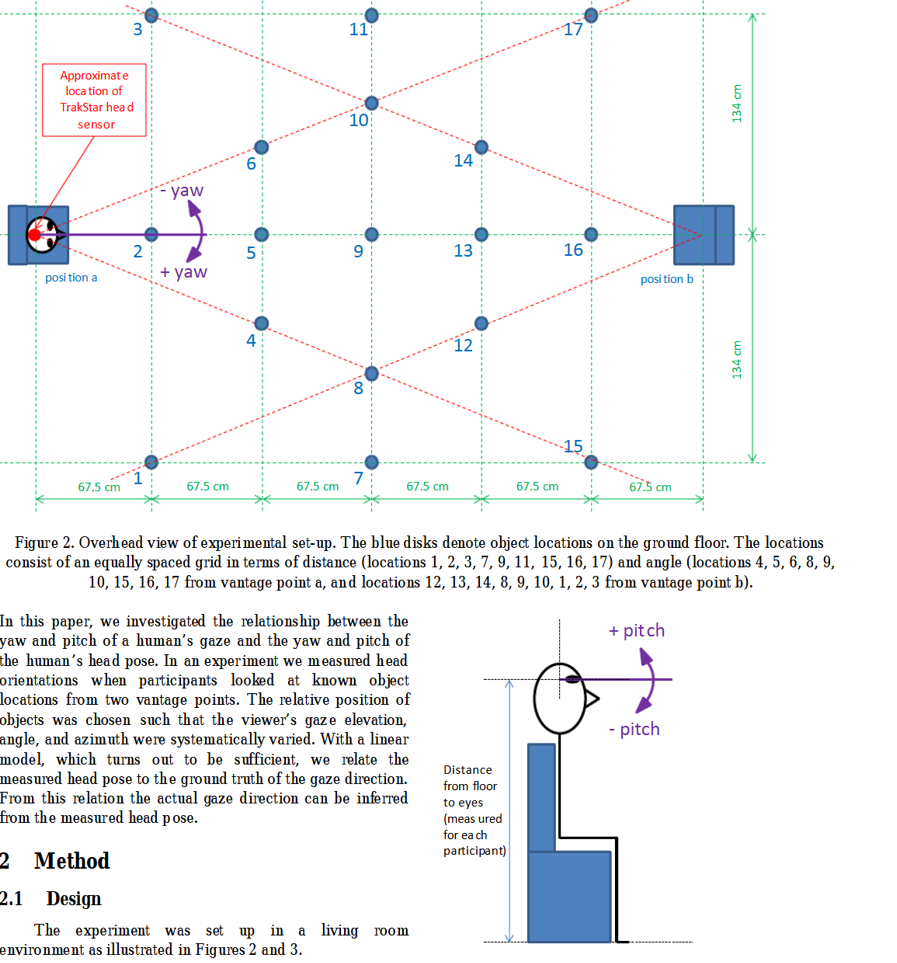
\includegraphics[width=0.7\textwidth]{eye-track-cursor/fig/gaze_definition.png}
    \caption{yawとpitchの定義}
    \label{fig:yaw_pitch_measurement}
\end{figure}
しかし、結果は失敗に終わってしまいました。考えられる要因とその根拠としたことは以下の通りです。\\
$\blacksquare$\textbf{考えられる原因}
\begin{itemize}
    \item 使用したデータの視線角度範囲が狭く、±20°の範囲に限定されていたため
\end{itemize}
$\blacksquare$\textbf{根拠としたこと}
\begin{itemize}
    \item 訓練結果によると学習時のロスは少なく、テスト時においても少なかった
\end{itemize}
\subsection{視線の角度推定(手法2)}
手法2においては、画像から直接視線の角度を推定する外部モデル(AxGazeEstimation)を活用しました。モデルの推論の流れや実験結果などは以下の通りです。\\
$\blacksquare$\textbf{視線推定モデル(AxGazeEstimation)による推論の流れ}
\begin{enumerate}
    \item BlazeFace\cite{bazarevsky2019blazeface}によって顔とその特徴点(目や鼻など)を検出
    \item 1.にて検出した顔とその特徴点を用いて、ResNetの縮小版(stage3モデル)によって視線角度を推定
\end{enumerate}

$\blacksquare$\textbf{結果}
\begin{itemize}
    \item 視線角度の推定に成功しました。(\ref{fig:gaze_direction_estimation_success})
\end{itemize}

\begin{figure}[!ht]
    \centering
    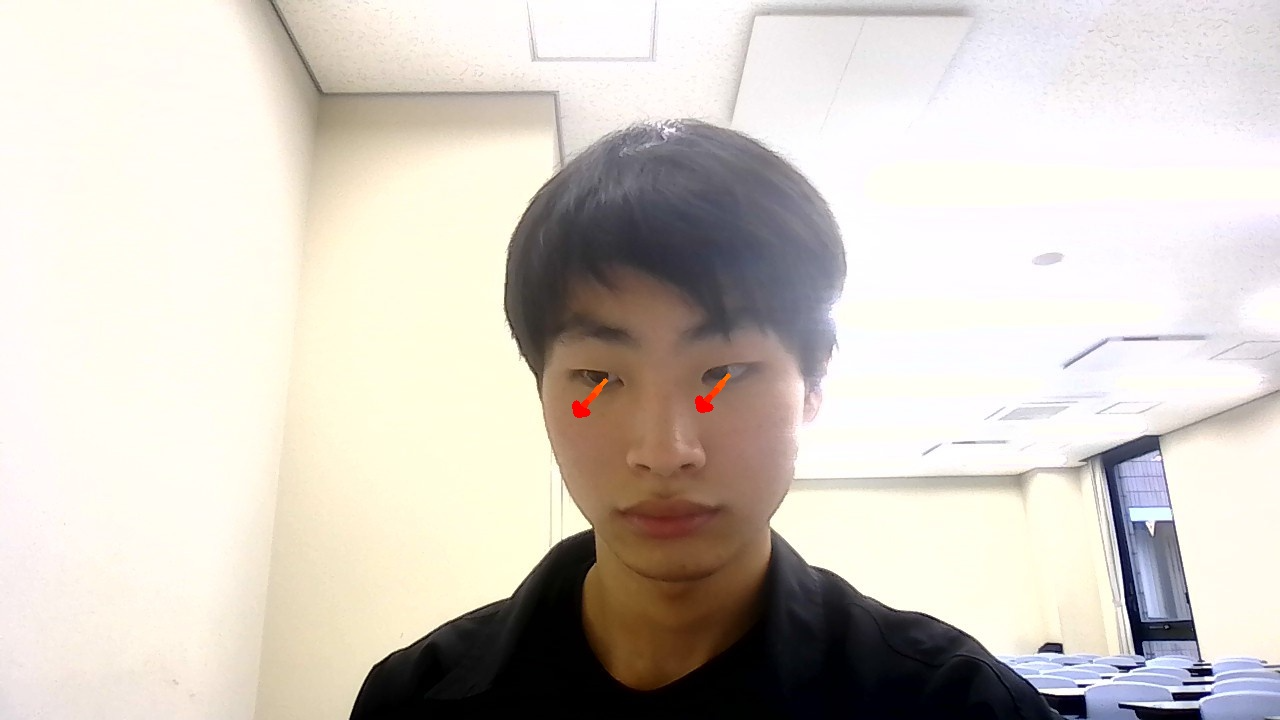
\includegraphics[width=0.7\textwidth]{eye-track-cursor/fig/gaze_direction_result.png}
    \caption{視線角度推定の結果}
    \label{fig:gaze_direction_estimation_success}
\end{figure}
この結果から、視線の角度推定では手法2を採用することにいたしました。
\section{最終結果}
1.2章にて言及した手順を用い、1.3~1.4章にて言及したモデルを用いることで、見ている場所をリアルタイムで推測できるモデルを開発できました。そして、\ref{fig:gaze_estimation_success}のように視線の位置をとらえることができました。\\

\begin{figure}[!ht]
    \centering
    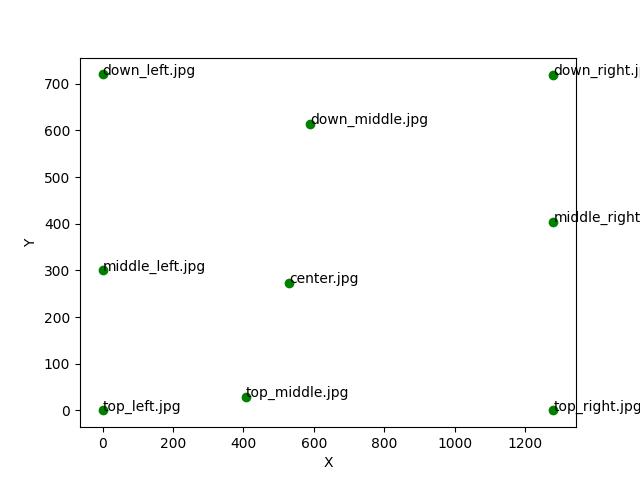
\includegraphics[width=0.7\textwidth]{eye-track-cursor/fig/gaze_at_result.png}
    \caption{視線角度推定の最終結果}
    \label{fig:gaze_estimation_success}
\end{figure}
※画面上のx座標・y座標におけるPCとの関係性は\ref{fig:definition_coordinates}です。
\begin{figure}[!ht]
    \centering
    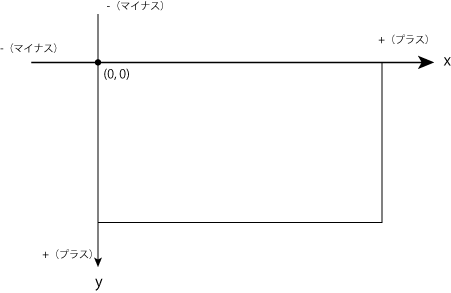
\includegraphics[width=0.7\textwidth]{eye-track-cursor/fig/pc_definition.png}
    \caption{PC上のスクリーン座標系 (x: 0~1280, y: 0~720)}
    \label{fig:definition_coordinates}
\end{figure}
\section{さいごに}
最終的にモデルを作成できましたが、第1.4.1章で考案した手法ではうまくいきませんでした。しかし、データに問題があるのかもしれないと考えられます。このことから、モデルだけでなく、データもきちんと選定する重要性があることが分かりました。\\
他にも様々なyaw,pitchに関する学習モデルが存在し、yaw,pitchの範囲が広い学習データもありましたが、どのデータもデータサイズが大きく、ダウンロードしにくい状況でした。そのため、今後はモデルについて考察するだけでなく、データ選定の手法についても学ぶ必要があることが分かりました。\\
また、今後はデータのyawやpitchの範囲が-20°~20°と狭いことが影響している可能性があるため、yawやpitchが±20°に近い角度のデータの比重を高め、モデルが広範囲の視線角度に対しても正確に推定できるようにして実験したいです。\\
\begin{figure}[!ht]
    \centering
    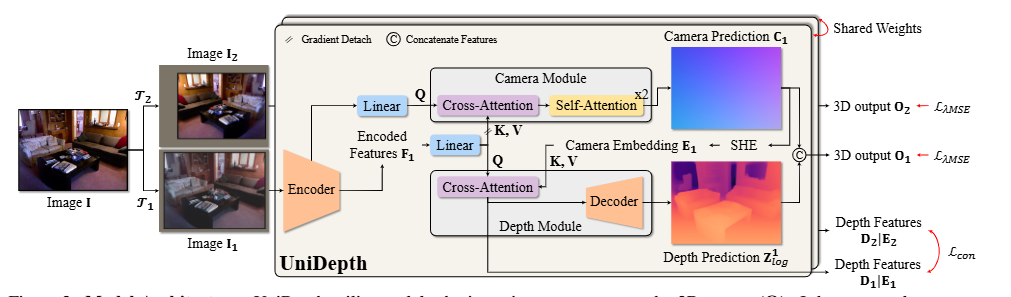
\includegraphics[width=0.7\textwidth]{eye-track-cursor/fig/UniDepth.png}
    \caption{UniDepthの構造}
    \label{fig:UniDepth}
\end{figure}
また、深度推定においてUniDepth(\ref{fig:UniDepth})などの様々な深度推定モデルがございました。そのため、今後はそういったモデルによって目とカメラの距離を求め、それを元に目とカメラとの位置関係を求めるようにしていきたいです。
